\section{Introduction to Operating Systems}

\paragraph{What's an OS?}
The OS is a layer between applications and hardware to ease development.
\begin{itemize}
	\item \textbf{Abstraction}. provides abstraction for applications:
		\begin{itemize}
			\item manages + hides hardware details
			\item uses low-level interfaces (not available to applications)
			\item multiplexes hardware to multiple programs (\emph{virtualization})
			\item makes hardware use efficient for applications
		\end{itemize}
	\item \textbf{Protection}.
		\begin{itemize}
			\item from processes using up all resources (\emph{accounting}, \emph{allocation})
			\item from processes writing into other processes memory
		\end{itemize}
	\item \textbf{Resource Management}.
		\begin{itemize}
			\item manages + multiplexes hardware resources
			\item decides between conflicting requests for resource use
			\item \emph{goal}: efficient + fair resource use
		\end{itemize}
	\item \textbf{Control}.
		\begin{itemize}
			\item controls program execution
			\item prevents errors and improper computer use
		\end{itemize}
	\item $ \leadsto $ \textbf{no universally accepted definition}
\end{itemize}

\paragraph{Hardware Overview}
\begin{itemize}
	\item \textbf{Bus}: CPU(s)/devices/memory (conceptually) connected to common bus
	\begin{itemize}
		\item CPU(s)/devices competing for memory cycles/bus
		\item all entities run concurrently
		\item \emph{today}: multiple buses
	\end{itemize}
	\item \textbf{Device controller}: has local buffer and is in charge of particular device
	\item \textbf{Interplay}:
	\begin{enumerate}
		\item CPU issues commands, moves data to devices
		\item Device controller informs APIC that it has finished operation
		\item APIC signals CPU
		\item CPU receives device/interrupt number from APIC, executes handler 
	\end{enumerate}
	\begin{figure}[h]\centering\label{BusSystem}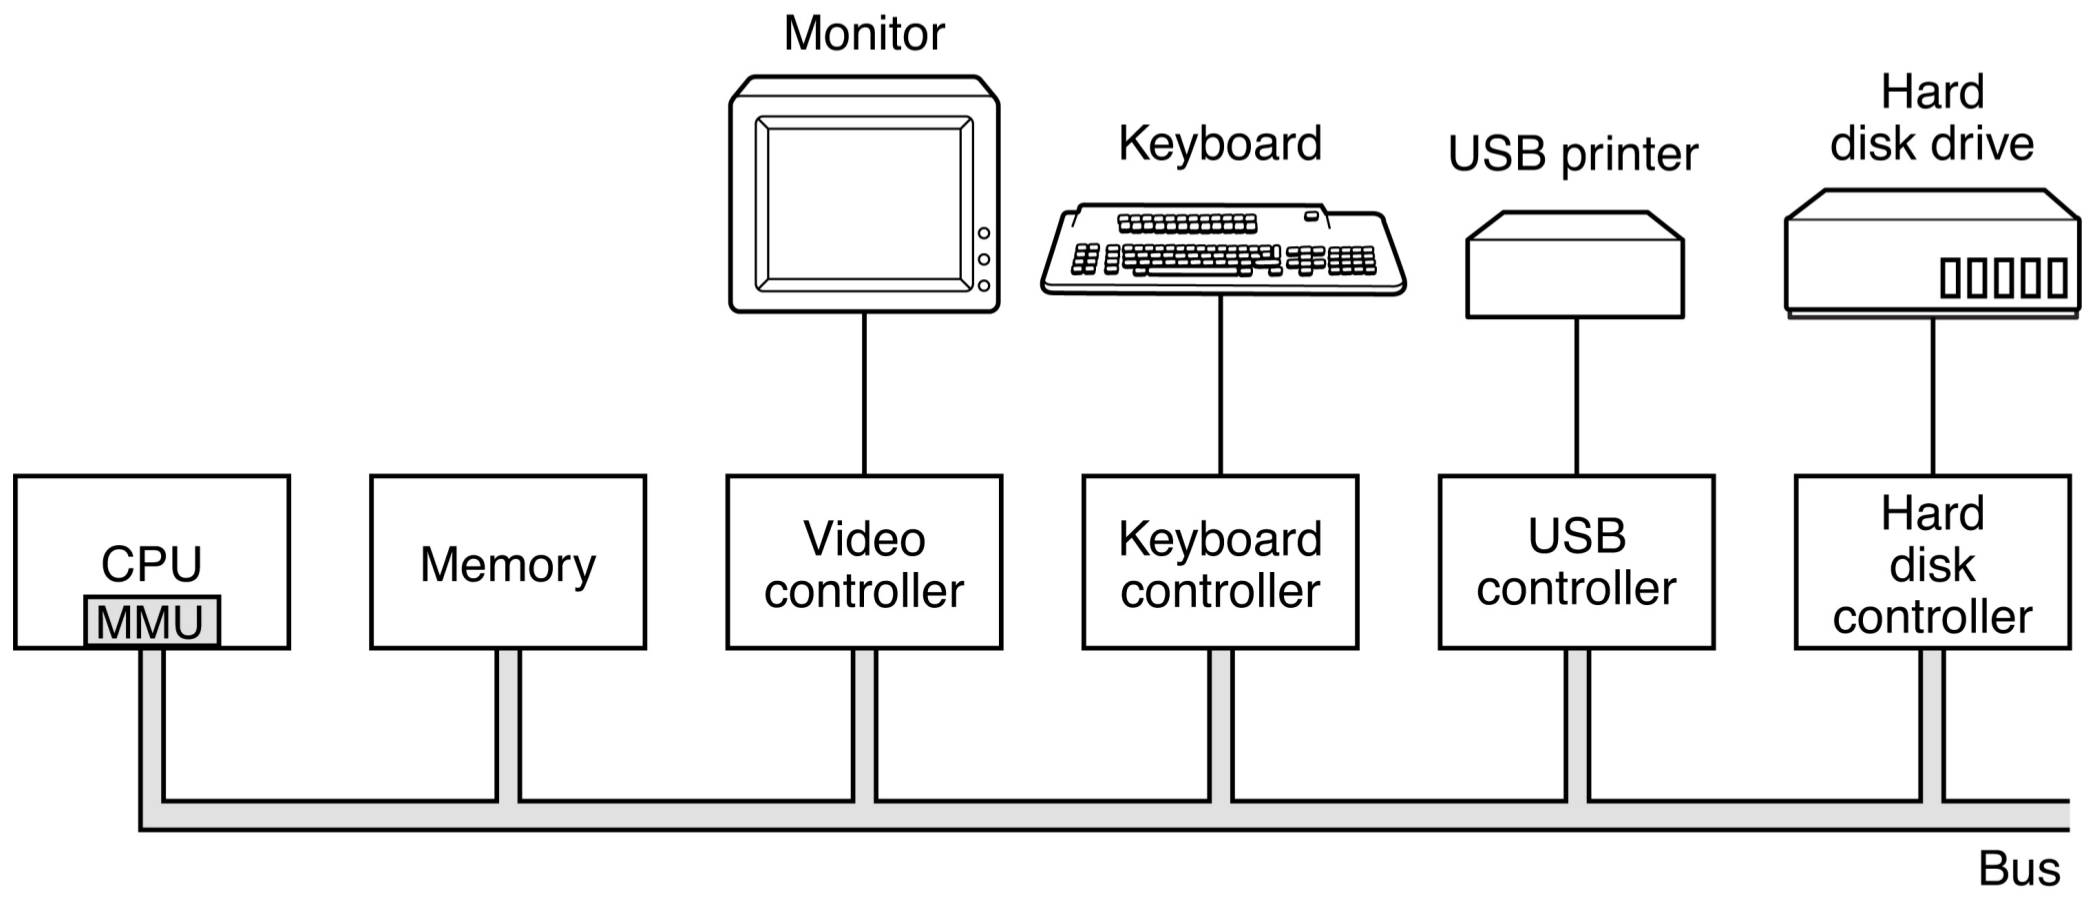
\includegraphics[width=0.33\textwidth]{BusSystem}\caption{Traditional bus design}\end{figure}
	\begin{figure}[h]\centering\label{BusSystemToday}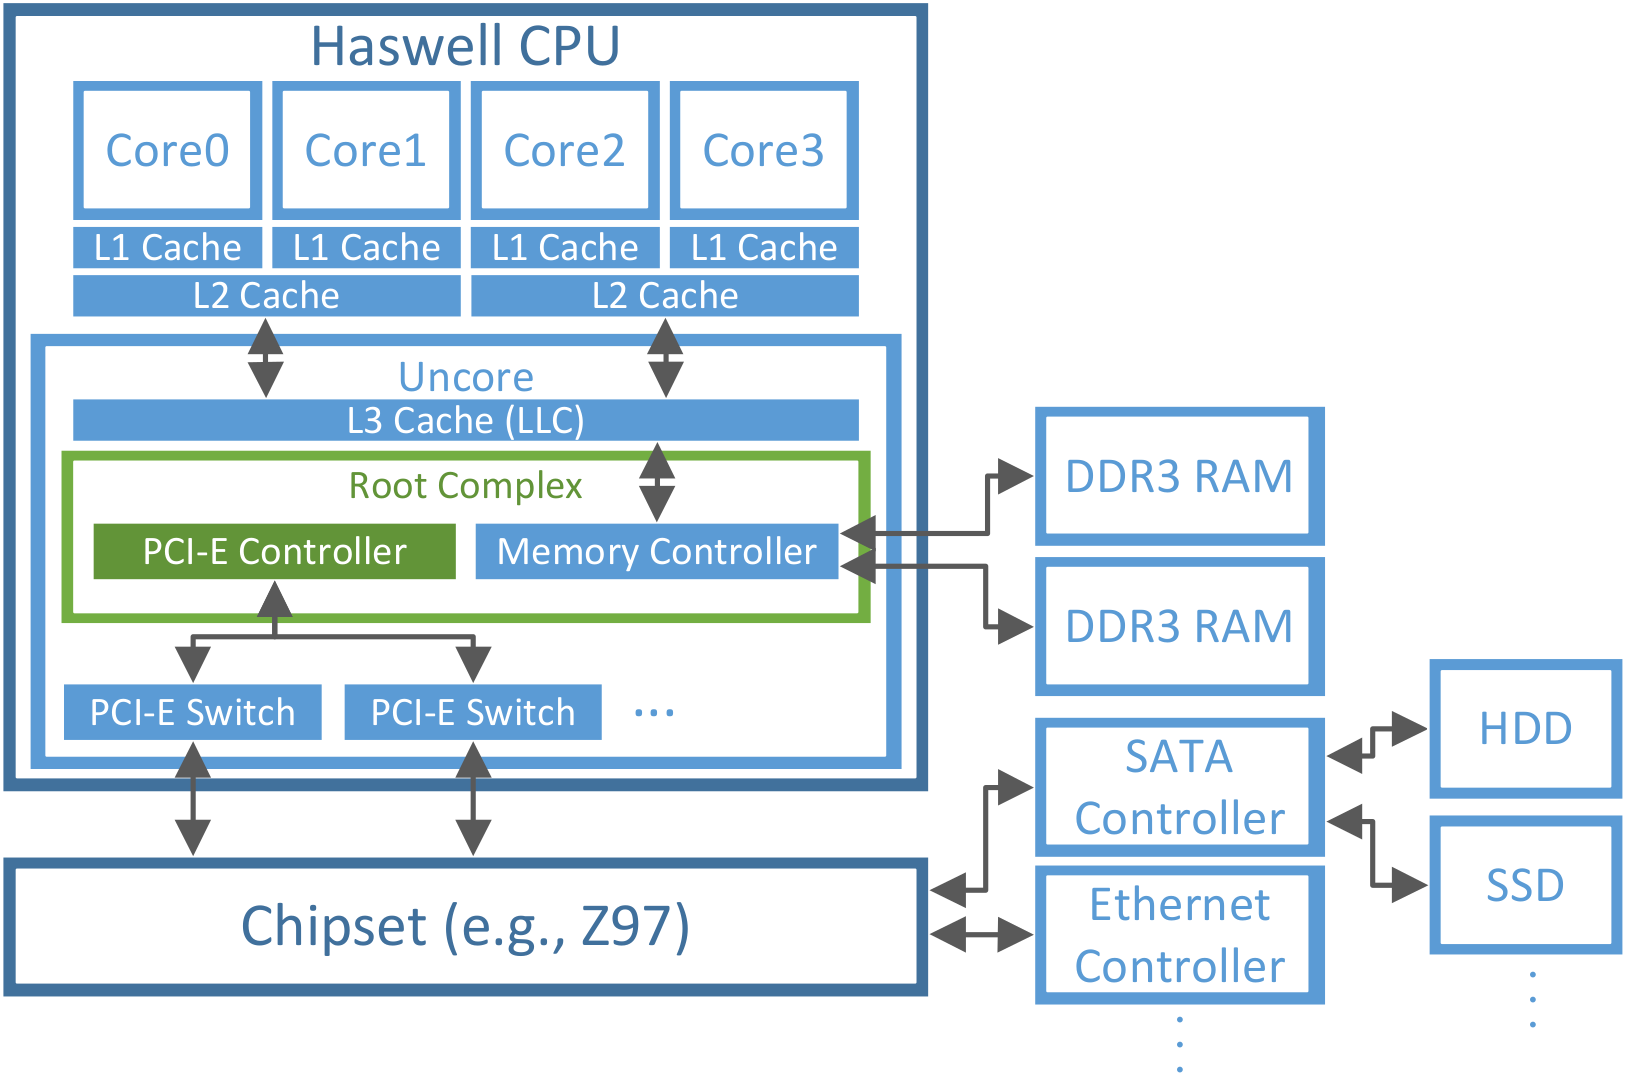
\includegraphics[width=0.33\textwidth]{BusSystemToday}\caption{Modern bus design}\end{figure}
\end{itemize}

\paragraph{Central Processing Unit (CPU) --- Operation}
\begin{itemize}
	\item \textbf{Principle}:
	\begin{enumerate}
		\item \emph{fetches} instructions from memory,
		\item \emph{executes} them
	\end{enumerate}
	\item \textbf{During execution}: (meta-)data is stored in CPU-internal registers, i.e.
	\begin{itemize}
	 	\item general purpose registers
	 	\item floating point registers
	 	\item instruction pointer (IP)
	 	\item stack pointer (SP)
	 	\item program status word (PSW)
	 \end{itemize}
\end{itemize}

\paragraph{CPU --- Modes of Execution}
\begin{itemize}
	\item \textbf{User mode} (x86: \emph{Ring 3}/\emph{CPL 3}):
		\begin{itemize}
			\item only non-privileged instructions may be executed
			\item cannot manage hardware $ \to $ \emph{protection}
		\end{itemize}
	\item \textbf{Kernel mode} (x86: \emph{Ring 0}/\emph{CPL 0}):
		\begin{itemize}
			\item all instructions allowed
			\item can manage hardware with \emph{privileged instructions}
		\end{itemize}
		\begin{figure}[h]\centering\label{OperationModes}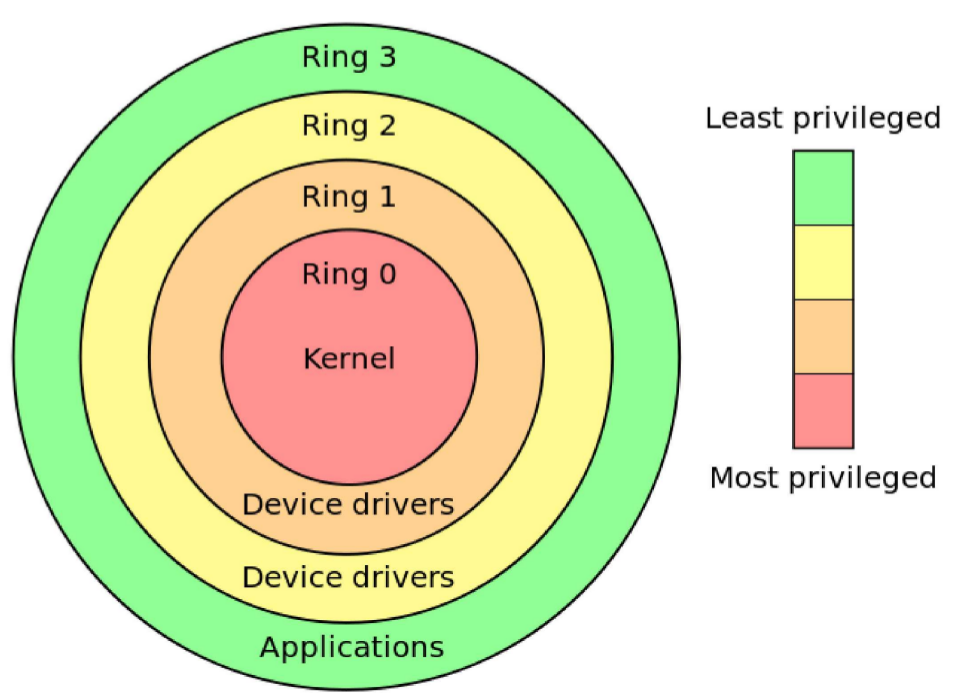
\includegraphics[width=0.2\textwidth]{OperationModes}\caption{The different protection layers in the \emph{ring model}}\end{figure}
\end{itemize}

\paragraph{Random Access Memory (RAM)}
\begin{itemize}
	\item \textbf{Principle}: keeps currently executed instructions + data
	\item \textbf{Connectivity}:
	\begin{itemize}
		\item \emph{today}: CPUs have built-in \textbf{memory controller} 
		\item \emph{CPU caches}: ``wired'' to CPU
		\item \emph{RAM}: connected via pins
		\item \emph{PCI-E switches}: connected via pins
	\end{itemize}
\end{itemize}

\paragraph{Caches}
\begin{itemize}
	\item \textbf{Problem}: RAM delivers instructions/data slower than CPU can execute
	\item \textbf{Locality principle}:
	\begin{itemize}
		\item \emph{spatial locality}: future refs often near previous accesses (e.g. next byte in array)
		\item \emph{temporal locality}: future refs often at previously accessed ref (e.g. loop counter)
	\end{itemize}
	\item \textbf{Solution}: \emph{caching} helps mitigating this memory wall
	\begin{enumerate}
		\item \emph{copy} used information temporarily from slower to faster storage
		\item \emph{check} faster storage first before going down \emph{memory hierarchy} 
		\item if \emph{not found}, data is copied to cache and used from there
	\end{enumerate}
	\item \textbf{Access latency}:
	\begin{itemize}
		\item \emph{register}: $ \sim $1 CPU cycle
		\item \emph{L1 cache} (per core): $ \sim $4 CPU cycles
		\item \emph{L2 cache} (per core pair): $ \sim $12 CPU cycles
		\item \emph{L3 cache/LLC} (per uncore): $ \sim $28 CPU cycles ($ \sim $25 GiB/s) 
		\item \emph{DDR3-12800U RAM}: $ \sim $28 CPU cycles + $ \sim $ 50ns ($ \sim $12 GiB/s)
	\end{itemize}
\end{itemize}

\paragraph{Device controlling}
\begin{itemize}
	\item \textbf{Device controller}: controls device, accepts commands from OS via \emph{device driver}
	\item \textbf{Device registers/memory}:
	\begin{itemize}
		\item \emph{control} device by writing device registers
		\item \emph{read} status of device by reading device registers
		\item \emph{pass data} to device by reading/writing device memory
	\end{itemize}
	\item \textbf{Device registers/memory access}:
	\begin{enumerate}
		\item \textbf{port-mapped IO} (PMIO): use special CPU instructions to access port-mapped registers/memory
		\item \textbf{memory-mapped IO} (MMIO):
		\begin{itemize}
			\item use same address space for RAM and device memory
			\item some addresses map to RAM, others to different devices
			\item access device's memory region to access device registers/memory
		\end{itemize}
		\item \textbf{Hybrid}: some devices use hybrid approaches using both
	\end{enumerate}
\end{itemize}

\begin{summary}
	\begin{itemize}
		\item The OS is an abstraction layer between applications and hardware (multiplexes hardware, hides hardware details, provides protection between processes/users)
		\item The CPU provides a separation of User and Kernel mode (which are required for an OS to provide protection between applications)
		\item CPU can execute commands faster than memory can deliver instructions/data --- memory hierarchy mitigates this memory wall, needs to be carefully managed by OS to minimize slowdowns
		\item device drivers control hardware devices through PMIO/MMIO
		\item Devices can signal the CPU (and through the CPU notify the OS) through interrupts
	\end{itemize}
\end{summary}
